\documentclass{article}
\usepackage[letterpaper]{geometry}
\geometry{verbose,tmargin=1in,bmargin=1in,lmargin=1in,rmargin=1in}

\usepackage[utf8]{inputenc}
\usepackage{amsmath}
\usepackage{listings}
\usepackage{graphicx}
\usepackage{enumitem}
\usepackage{amssymb}
\usepackage{tabularx}
\usepackage{hyperref}
\usepackage{caption}
\usepackage{float}
\usepackage[section]{placeins}
\usepackage{empheq}
\usepackage{stackengine}
\usepackage{subcaption}
\usepackage{array}
\usepackage[super]{nth}

\def\delequal{\mathrel{\ensurestackMath{\stackon[1pt]{=}{\scriptstyle\Delta}}}}


\title{CIS 680: Project 1 Part A}
\author{Junfan Pan}
\date{09/13/2020}

\begin{document}
    \maketitle
    
    \section{Plot Loss and Gradient}
    \noindent
    \begin{enumerate}
    	\item[1.1] 
    	Sigmoid Activation Function\\
    	\begin{minipage}[t]{\linewidth}
        	\captionsetup{type=figure}
            \centering
            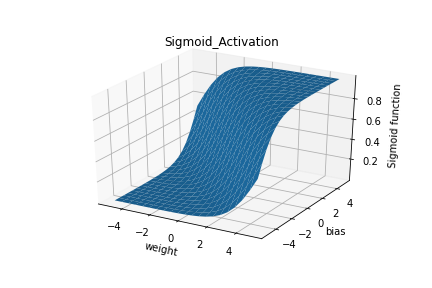
\includegraphics[width=0.65\linewidth]{Sigmoid_Activation.png}
            \caption{Sigmoid Function}
            \label{fig: Sigmoid Function}  
        \end{minipage}
        
        \item[1.2] 
    	L2 Loss\\
    	\begin{minipage}[t]{\linewidth}
        	\captionsetup{type=figure}
            \centering
            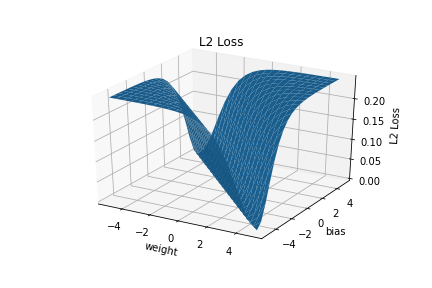
\includegraphics[width=0.65\linewidth]{L2 Loss.png}
            \caption{L2 Loss} 
            \label{L2 Loss}    
        \end{minipage}
        
        \newpage
        \item[1.3] 
    	L2 Loss Gradient\\
    	\begin{minipage}[t]{\linewidth}
        	\captionsetup{type=figure}
            \centering
            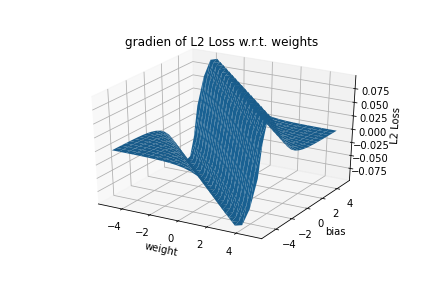
\includegraphics[width=0.65\linewidth]{gradien of L2 Loss w.r.t. weights.png}
            \caption{L2 Loss Gradient} 
            \label{L2 Loss Gradient}     
        \end{minipage}
        
        \item[1.4] 
    	Cross Entropy Loss\\
    	\begin{minipage}[t]{\linewidth}
        	\captionsetup{type=figure}
            \centering
            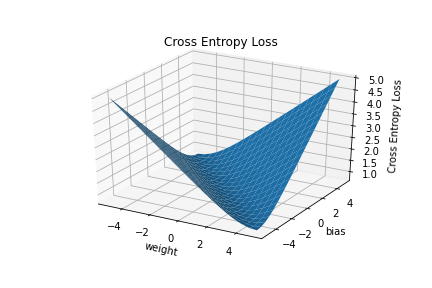
\includegraphics[width=0.65\linewidth]{Cross Entropy Loss.png}
            \caption{Cross Entropy Loss} 
            \label{Cross Entropy Loss}     
        \end{minipage}
        
        \item[1.5] 
    	Cross Entropy Gradient\\
    	\begin{minipage}[t]{\linewidth}
        	\captionsetup{type=figure}
            \centering
            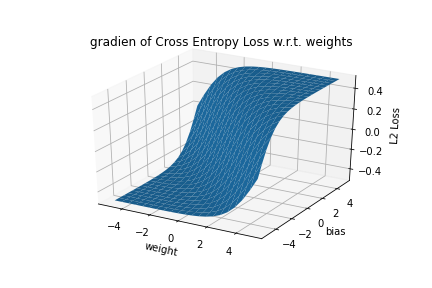
\includegraphics[width=0.65\linewidth]{gradien of Cross Entropy Loss w.r.t. weights.png}
            \caption{Cross Entropy Gradient} 
            \label{Cross Entropy Gradient}     
        \end{minipage}
        
        \item[1.6]
        \begin{itemize}
        	\item
        	What's the difference between cross-entropy loss and L2 loss?\\
        	From the z coordinates of Figure \ref{L2 Loss} and Figure \ref{Cross Entropy Loss}, we can observe that in terms of the same value of weight and bias, the cross-entropy loss is much larger than L2 loss. In addition, the increment of cross-entropy which corresponds to the same amount of increment of weight and bias is much larger than this of L2 loss. Finally, the cross-entropy loss keep growing while the there is no obvious increase of L2 loss when the weight and bias reach some threshold.\\
        	
        	\item
        	What's
the difference between the gradients from cross-entropy loss and L2 loss?\\
        	From Figure \ref{L2 Loss Gradient} and Figure \ref{Cross Entropy Gradient}, we can see that the gradient of L2 loss is almost zero when the weight and bias are large. This means that the model learns little at the very start when the output is far from target. By comparing, the gradient of cross-entropy loss is stable and large which facilitates fast training of the model.\\

        	
        	\item
        	Predict how these differences will influence the efficiency of learning?\\
        	Considering that the gradient of cross-entropy is much larger than the gradient of L2 loss under the same condition and especially at the start of training when error is large, therefore using the cross-entropy Loss can have better performance in achieving higher efficiency in training the model.\\

        \end{itemize}
    	
    \end{enumerate} 
    
    
    \section{Solving XOR with a 2-layer Perceptron}
    \noindent
    \begin{enumerate}
    	\item[2.1] Formulate the XOR approximation as an optimization problem using cross entropy loss. See below.
    	 \begin{figure}[H]
     	\centering
         	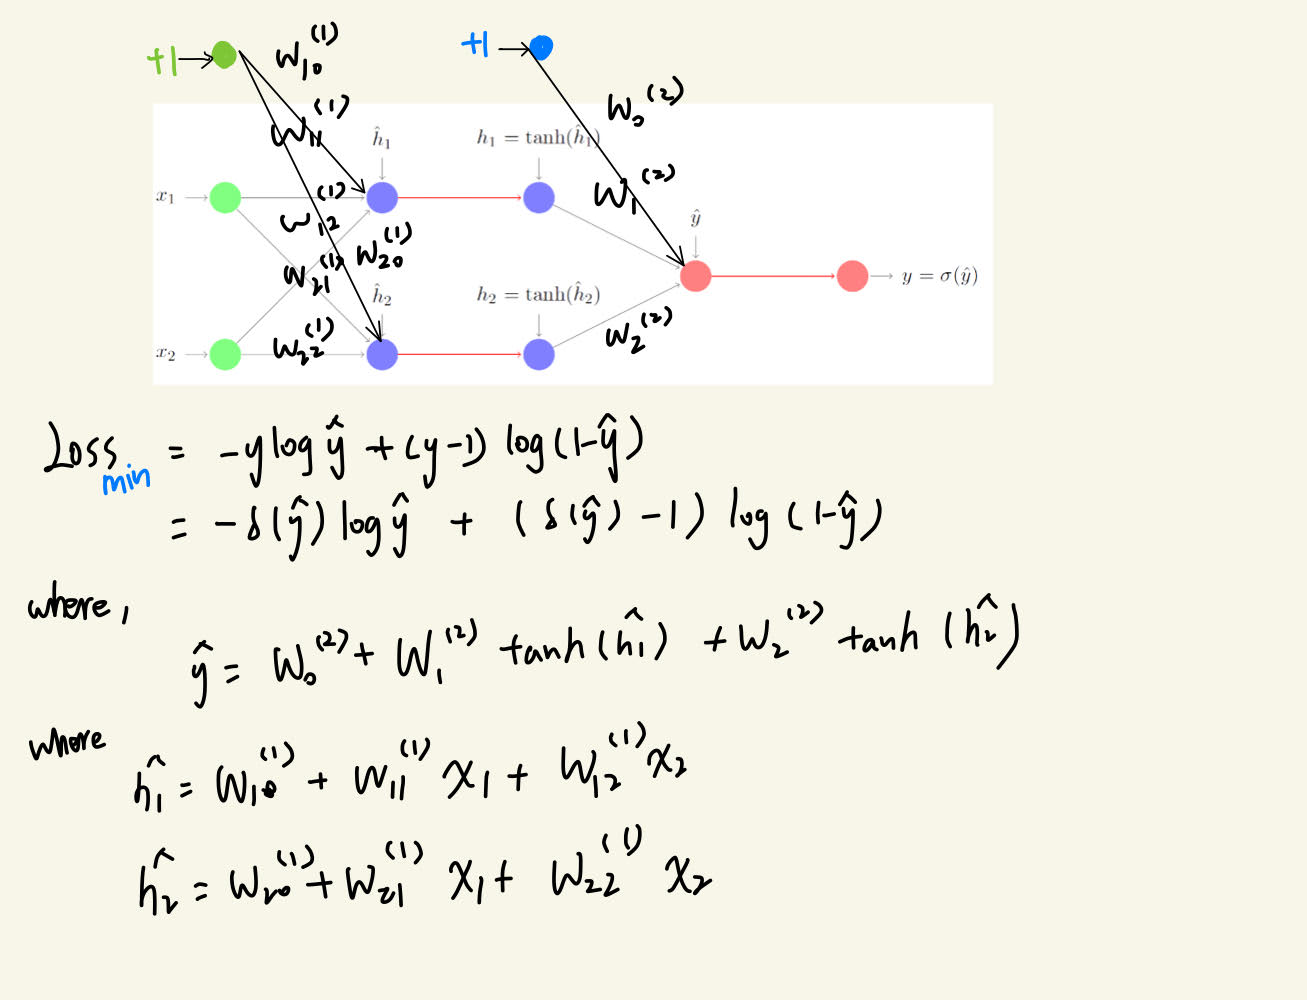
\includegraphics[width=\textwidth]
         	{optimization.jpg}
     	\end{figure}
     	
    	\item[2.2] 
        The decision boundaries of different epochs are shown below:\\
        \begin{figure}[H]
        
     	\centering
     	\begin{subfigure}[b]{0.45\textwidth}
         	\centering
         	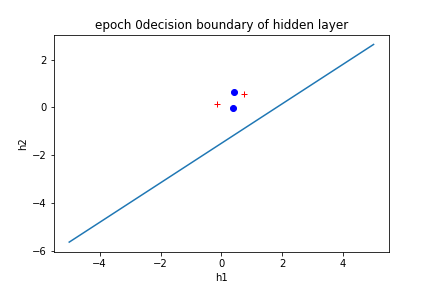
\includegraphics[width=\textwidth]
         	{epoch 0 decision boundary of hidden layer.png}
         	\caption{Decision Boundary at Epoch 0}
         	\label{fig:Hyperplane Epoch 0}
     	\end{subfigure}
     	\hfill
     	\begin{subfigure}[b]{0.45\textwidth}
         	\centering
         	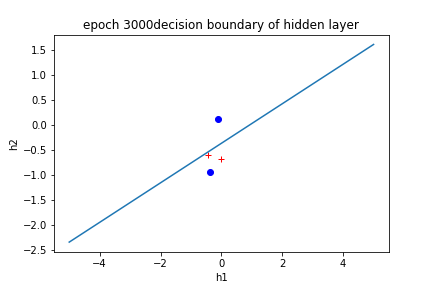
\includegraphics[width=\textwidth]
         	{epoch 3000 decision boundary of hidden layer.png}
         	\caption{Decision Boundary at Epoch 3000}
         	\label{fig:Hyperplane Epoch 1000}
     	\end{subfigure}
     	\end{figure}
     	
     	
     	\begin{figure}[H]
     	\centering
     	\begin{subfigure}[b]{0.45\textwidth}
         	\centering
         	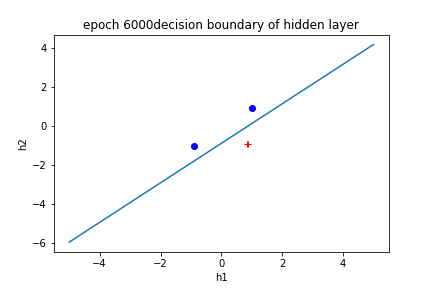
\includegraphics[width=\textwidth]
         	{epoch 6000 decision boundary of hidden layer.png}
         	\caption{Decision Boundary at Epoch 6000}
         	\label{fig:Hyperplane Epoch 2000}
     	\end{subfigure}
     	\hfill
     	\begin{subfigure}[b]{0.45\textwidth}
         	\centering
         	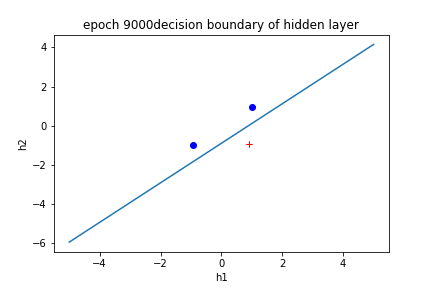
\includegraphics[width=\textwidth]
         	{epoch 9000 decision boundary of hidden layer.png}
         	\caption{Decision Boundary at Epoch 9000}
         	\label{fig:Hyperplane Epoch 3000}
     	\end{subfigure}
		
		\end{figure}
		
		The red cross represents (0,0) and (1,1) while the blue dot represents (0,1) and (1,0).
		
		\item[2.3] The network can not generate a single decision boundary to implement XOR. The reason is that if there is no activation function of the hidden layer, then the hidden layer will be a linear function. Therefore, the first layer plus the hidden layer are actually a single layer while it is known to all that it is impossible to achieve XOR using a single layer, which is actually a linear function.\\\\
		
    \end{enumerate}
    
    \section{Train a Convolutional Neural Network}
    \noindent
    \begin{enumerate}
    	\item[3.1] See Python code in the colab notebook.
    	\item[3.2] The learning curves are shown below:
    	\begin{figure}[H]
        
     	\centering
     	\begin{subfigure}[b]{0.45\textwidth}
         	\centering
         	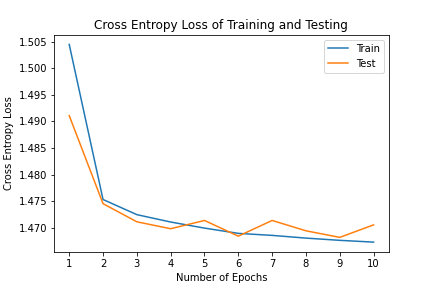
\includegraphics[width=\textwidth]
         	{Cross Entropy Loss of Training and Testing.png}
         	\caption{MNIST Loss}
         	\label{fig:MNIST Loss}
     	\end{subfigure}
     	\hfill
     	\begin{subfigure}[b]{0.45\textwidth}
         	\centering
         	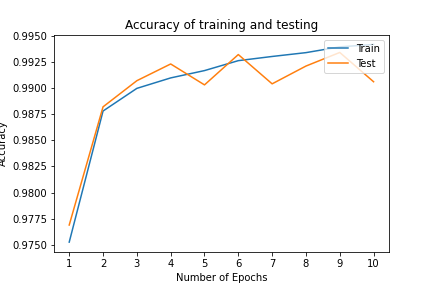
\includegraphics[width=\textwidth]
         	{Accuracy of training and testing.png}
         	\caption{MNIST Accuracy}
         	\label{fig:MNIST Accuracy}
     	\end{subfigure}
     	\end{figure}
     	
     	The model reaches 99\% accuracy on the test dataset since the \nth{3} epoch. 
    	
    \end{enumerate}
    
        
\end{document}  